\documentclass[10pt,landscape]{article}
\usepackage{multicol}
\usepackage{calc}
\usepackage{ifthen}
\usepackage[landscape]{geometry}
\usepackage{listings}
\usepackage{amsmath,amsthm,amsfonts,amssymb}
\usepackage{mathtools}
\usepackage{color,graphicx,overpic}
\usepackage{hyperref}
\usepackage[table, dvipsnames]{xcolor} % for \colorbox and named colors
\usepackage{transparent}

\usepackage{MnSymbol}
\usepackage{graphicx}
\usepackage{wrapfig}
\usepackage{tikz}

\usepackage{blindtext}

% This sets page margins to .1 inch if using letter paper, and to 1cm
% if using A4 paper. (This probably isn't strictly necessary.)
% If using another size paper, use default 1cm margins.
\ifthenelse{\lengthtest { \paperwidth = 11in}}
    { \geometry{top=0.2in,left=0.2in,right=0.2in,bottom=0.2in} }
    {\ifthenelse{ \lengthtest{ \paperwidth = 297mm}}
        {\geometry{top=1cm,left=1cm,right=1cm,bottom=1cm} }
        {\geometry{top=1cm,left=1cm,right=1cm,bottom=1cm} }
    }

% Turn off header and footer
\pagestyle{empty}

% Redefine section commands to use less space
\makeatletter
\renewcommand{\section}{\@startsection{section}{1}{0mm}%
                                {-1ex plus -.5ex minus -.2ex}%
                                {0.5ex plus .2ex}%x
                                {\normalfont\large\bfseries}}
\renewcommand{\subsection}{\@startsection{subsection}{2}{0mm}%
                                {-1ex plus -.5ex minus -.2ex}%
                                {0.5ex plus .2ex}%
                                {\normalfont\normalsize\bfseries}}
\renewcommand{\subsubsection}{\@startsection{subsubsection}{3}{0mm}%
                                {-1ex plus -.5ex minus -.2ex}%
                                {0.5ex plus .2ex}%
                                {\normalfont\footnotesize\bfseries}}
\makeatother

% Itemize to use less space
\usepackage{enumitem}
\setlist{leftmargin=*, nosep}
\setenumerate{nosep}

% Define BibTeX command
\def\BibTeX{{\rm B\kern-.05em{\sc i\kern-.025em b}\kern-.08em
    T\kern-.1667em\lower.7ex\hbox{E}\kern-.125emX}}

% Don't print section numbers
\setcounter{secnumdepth}{0}


\setlength{\parindent}{0pt}
\setlength{\parskip}{0pt plus 0.5ex}

%My Environments
\newtheorem{example}[section]{Example}

\newcommand{\Blue}[1]{\noindent{\textcolor{Blue}{\textbf{#1}}}:}
\newcommand{\Red}[1]{\noindent{\textcolor{BrickRed}{\textbf{#1}}}:}
\newcommand{\Green}[1]{\noindent{\textcolor{PineGreen}{\textbf{#1}}}:}
\newcommand{\Hint}[1]{\noindent{\textcolor{Orange}{#1}}}

\newcommand*{\eg}{e.g.\@\xspace}
\newcommand*{\ie}{i.e.\@\xspace}
\newcommand*{\Eg}{E.g.\@\xspace}
\newcommand*{\Ie}{I.e.\@\xspace}
\newcommand*{\esp}{esp.\@\xspace}
\newcommand*{\wrt}{\ifmmode \stext{w.r.t.} \else w.r.t.\@\xspace \fi}


\usepackage{draftwatermark}
% Configure the watermark
\SetWatermarkText{Made with love by \texttt{junruren}} % Set the watermark text
\SetWatermarkScale{2.5}            % Adjust the scale of the watermark
\SetWatermarkLightness{0.9}      % Set the lightness (closer to 1 is more faded)
% -----------------------------------------------------------------------

\begin{document}
\raggedright
\scriptsize

\begin{multicols}{4}
% multicol parameters
% These lengths are set only within the two main columns
%\setlength{\columnseprule}{0.25pt}
\setlength{\premulticols}{1pt}
\setlength{\postmulticols}{1pt}
\setlength{\multicolsep}{1pt}
\setlength{\columnsep}{2pt}
\subsection{Net Present Value (NPV)}
\Blue{Discoint rate $r$} you're indifferent between receiving \$1 today and $\$\frac{1}{1+r}$ in one period.

\Blue{Present Value (PV)} \fbox{$PV(CF_t) = \frac{CF_t}{(1+r)^t}$}
how much a cash flow (CF) at time $t$ is worth at time 0 (today). Computing a PV is often called \Hint{``discounting''}.

\Red{NPV} \fbox{$NPV = \sum_{t=0}^{T} \frac{CF_t}{(1+r)^t}$} summs over PVs of all cash flows in a project.
\begin{itemize}
    \item \Green{Scalability} $NPV(\alpha CF_1, \dots, \alpha CF_T) = \alpha NPV(CF_1, \dots, CF_T)$
    \item \Green{Additivity} $NPV(X_1 + Y_1, \dots, X_T + Y_T) = NPV(X_1, \dots, X_T) + NPV(Y_1, \dots, Y_T)$
    \item \Green{Breaking up by time} $NPV(CF_1, \dots, CF_T) = NPV(CF_1, \dots, CF_j) + NPV(CF_{j+1}, \dots, CF_T)$
\end{itemize}

\Blue{Future Value (FV)}
\fbox{{$FV_T(CF_0) = CF_0(1+r)^T$}}
how much a cash flow at time 0 (today) is worth in $T$ periods.

\Blue{Perpetuity}
\begin{itemize}
    \item \underline{Constant} recurring cash flow $A$ forever starting \textbf{1 period from now}: \fbox{$PV = \frac{A}{r}$}
    \item \underline{Growing} perpetuity starting \textbf{1 period from now} with cash flow $A$, growth rate $g$: \fbox{$PV = \frac{A}{r-g} (r > g)$}
\end{itemize}

\Blue{Annuity}
\begin{itemize}
    \item \underline{Constant} recurring cash flow $A$ for $T$ periods starting \textbf{1 period from now}:
        \Hint{(\Eg a loan)}
        \fbox{$PV = \frac{A}{r} \left(1 - \frac{1}{(1+r)^T}\right)$}
        \fbox{$FV = PV \cdot (1+r)^T = A \frac{(1+r)^T - 1}{r}$}
    \item \underline{Growing} annuity starting \textbf{1 period from now} with cash flow $A$, growth rate $g$ for $T$ periods.
        \begin{itemize}
            \item If $r \neq g$
                \fbox{$PV = \frac{A}{r-g} \left(1 - \frac{(1+g)^T}{(1+r)^T}\right)$};
                \fbox{$FV = A \left(\frac{(1+r)^T - (1+g)^T}{r-g}\right)$}
            \item If $r = g$
                \fbox{$PV = T \left(\frac{A}{1+r}\right)$};
                \fbox{$FV = T \cdot A \cdot (1+r)^{T-1}$}
        \end{itemize}
\end{itemize}

\Red{Annual Percentage Rate (APR) \& Effective Annual Rate (EAR)}
\fbox{$(1+EAR) = \left(1 + \frac{APR}{k}\right)^k = (1 + r)^k$}
where $k$ is the number of compounding periods per year and $r$ is the per-period (\eg monthly) interest rate.
\begin{itemize}
    \item \underline{APR} $= r \cdot k$
    \item \underline{EAR} \ie Annual Percentage Yield (APY)
\end{itemize}

\subsubsection{Mortgage-related terms}

\Blue{Principal} the amount of \$ \underline{borrowed} in a lending agreement.
\Eg Buy a \$1,000,000 house with a 20\% down payment, the principal is \$800,000.

\Blue{Interest}
\begin{itemize}
    \item \Green{Fixed rate} No matter what happens to interest rates around the world, you would still be charged
        interest at this same rate.
    \item \Green{Adjustable rate (ARM)} \Eg an adjustable rate of 3\% \underline{above} the federal funds rate (the
        Fed's benchmark rate). If this rate is around 4.5\%, you would be charged a 7.5\% interest rate. If in the next
        month the Fed raises to 5\%, you would be charged an 8\% interest rate.
\end{itemize}

\Blue{Amortization schedule} sequence of payments made through the loan's lifetime. A part of the payments goes to
reduce (\ie amortize) the principal owed, and the rest goes to pay the interest on the loan.

\Blue{Collateral} An asset offered by the borrower as a guarantee in a loan. If you fail to make payments, the bank can
take the collateral.

\Blue{Refinancing} Paying off an existing loan with a new loan that has better terms. \Eg lower interest rate, lower
monthly payment, shorter loan term.

\Green{\Eg} a 30-year fixed-rate mortgage, APR 9\% compounded monthly. Fixed monthly payment $= \$3000$. First payment
will start next month and last until the contract expires in 30 years.
\begin{itemize}
    \item \Green{How much borrowed when took out the mortgage?}
        use the constant annuity formula, where
        \Hint{$A = \mathdollar 3000$, $r = \frac{0.09}{12} = 0.0075$, $T = 30 \times 12 = 360$}.
        $PV = \frac{A}{r} \left(1 - \frac{1}{(1+r)^T}\right) = \frac{3000}{0.0075} \left(1 - \frac{1}{(1+0.0075)^{360}}\right) = \mathdollar 372,845.60$
    \item \Green{10 years later, how much must pay back to the bank if sell the house?}
        (\ie NPV of the remaining principal amount as of this future date.)
        \Hint{$T = 20 \times 12 = 240$}
        $PV = \frac{3000}{0.0075} \left(1 - \frac{1}{(1+0.0075)^{240}}\right) = \mathdollar 333,434.86$
    \item \Green{Why the remaining principal is still so high after 10 years' worth of repayments?}
        \Hint{Because the amortization schedule is front-loaded.} \Ie Early on in the life of the mortgage, the vast majority
        of each monthly payment is interest: interest is applied to the remaining principal amount, and this remaining
        principal is highest in month 1 and decreases over time. Because the majority of each monthly payment in the
        early years is interest, the principal repayment amounts are small, and the remaining principal de-creases very
        slowly. (It's only toward the end of the mortgage that interest payments decline enough to repay the principal
        more quickly.)
\end{itemize}

\Red{Inflation $i$} the change in CPI \fbox{$1 + i_{t+1} = \frac{CPI_{t+1}}{CPI_t}$}
\begin{itemize}
    \item \Green{``Nominal''} \underline{not} adjusted for inflation
    \item \Green{``Real''} adjusted for inflation
\end{itemize}

\Blue{Real rate of return} $r_{\text{real}} = \frac{1 + r_{\text{nominal}}}{1 + i} - 1$
\fbox{$r_{\text{real}} \approx r_{\text{nominal}} - i$}

\Blue{Treat inflation consistently for NPV}

\fbox{$PV(CF_T) = \frac{CF_{\text{nominal,T}}}{(1 + r_{\text{nominal,T}})^T} = \frac{CF_{\text{real,T}}}{(1+r_{\text{real,T}})^T}$}
(``$_{,T}$'' denotes the cash flow at time $T$)

\subsection{Capital Budgeting}

To maximize value, take on \Hint{only projects with positive NPV}.
\begin{itemize}
    \item \Green{Single} take it only if it has positive NPV.
    \item \Green{Independent} take all with positive NPV.
    \item \Green{Mutually exclusive} take the one with the highest positive NPV.
    \item \Hint{Ignore} sunk costs, including opportunity costs.
\end{itemize}

\Red{\underline{Cash} operating expenses}
\begin{itemize}
    \item \Blue{COGS} direct costs attributable to the production of the goods sold by a business.
    \item \Blue{R\&D} costs associated with discovering new knowledge or develop new products, processes, and services.
    \item \Blue{SG\&A} costs not directly tied to the production of goods. \eg ``S'': advertising and sales commissions. ``G'': salaries of non-production personnel. ``A'': legal, accounting, and exec salaries.
\end{itemize}

\Blue{Depreciation} \underline{non-cash} expense that reduces the value of an asset over time. \Hint{For most finance
problems, we want to strip out effects of depreciation to get back to free cash flow.} Exception: if depreciation
affects free cash flows through taxes.

\Red{EBITDA} \fbox{$= (\text{Op. Rev.}) - (\text{All Op. Exp. w/o depreciation})$}

\Red{EBIT} \fbox{$= \text{EBITDA} - \text{Depreciation (\& Amort.)}$}

\Red{Cash Flows} from accounting statements
\fbox{$CF = (1 - \tau) (\text{EBITDA}) + \tau (\text{Dep.}) - (\text{CapEx}) - \Delta \text{WC}$}
\fbox{$CF = (1 - \tau) (\text{EBIT}) + (\text{Dep.}) - (\text{CapEx}) - \Delta \text{WC}$}

\Red{Working Capital (WC)} \fbox{$= \text{Inventory} + \text{A/R} - \text{A/P}$}
We are about \Hint{changes (\ie $\Delta$) in WC, not levels} because if keeping WC constant, no new cash flow required.

\subsubsection{Hotspur example}
\Hint{Not considering CF in year 0}
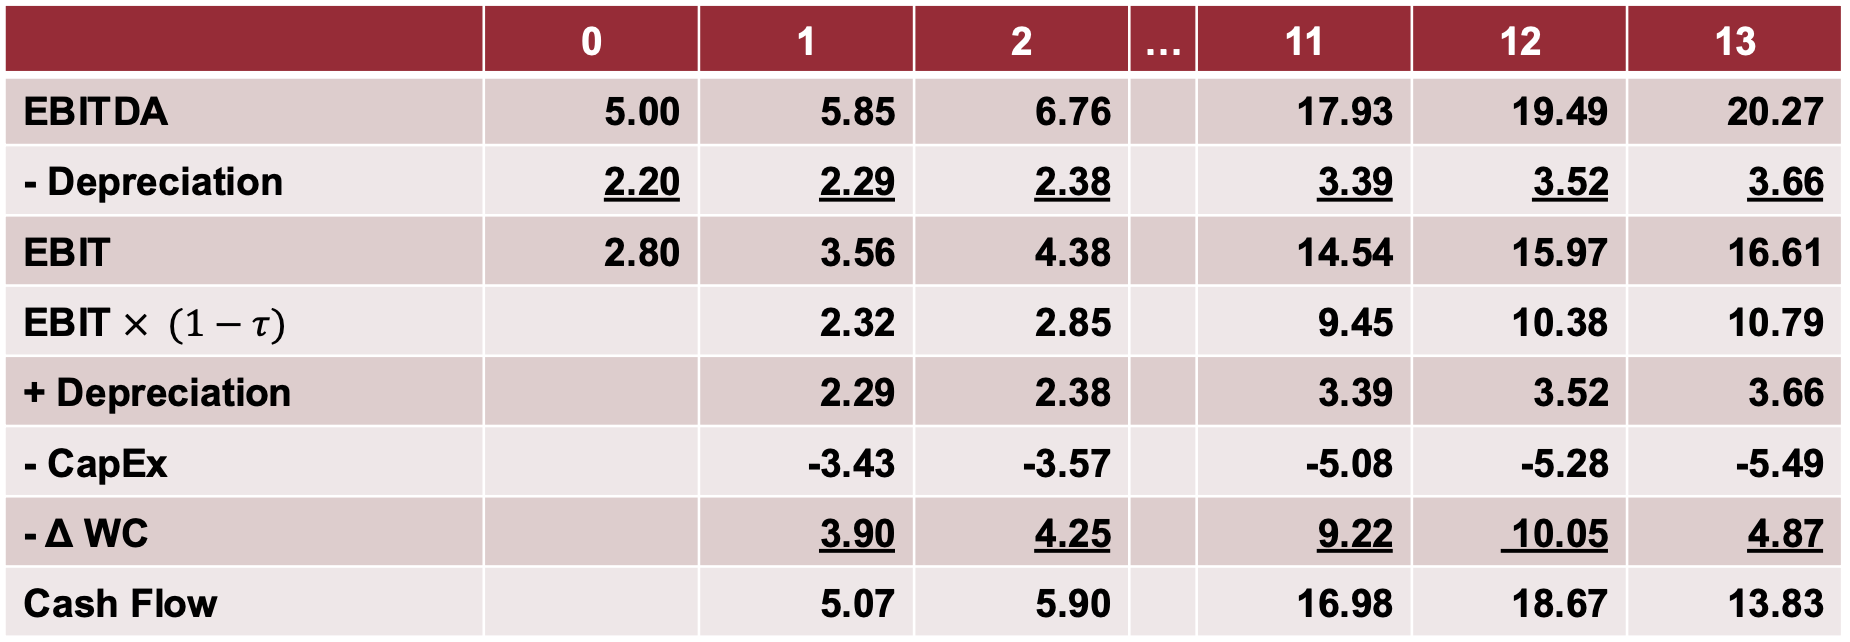
\includegraphics[width=\columnwidth]{CF.png}
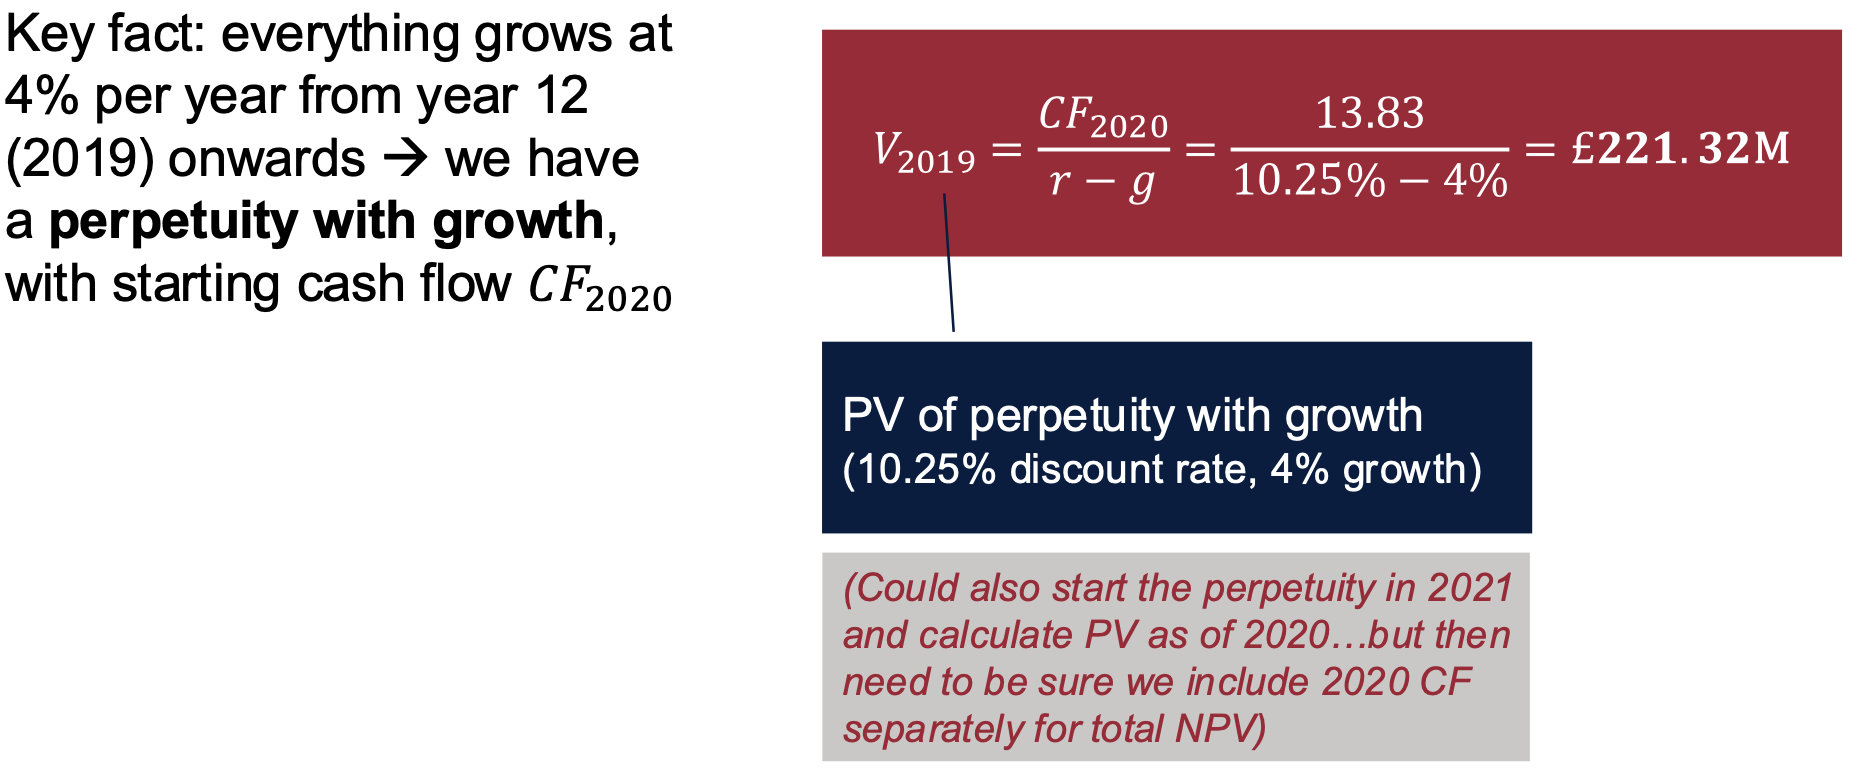
\includegraphics[width=\columnwidth]{Terminal.png}
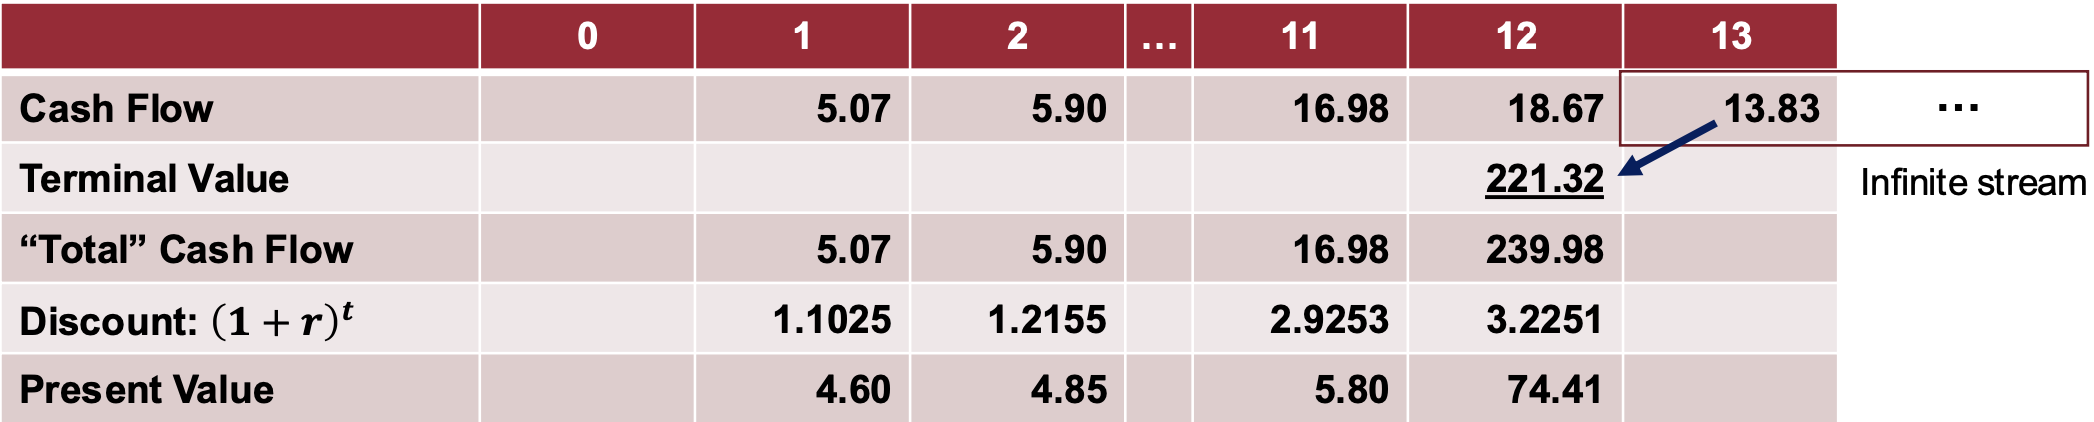
\includegraphics[width=\columnwidth]{DCF.png}
\Red{Enterprise Value (EV)} PV of future CFs
$EV = \sum_{t=1}^{\infty} PV(CF_t)$
\ie estimated via discounted CF (DCF) analysis.

\Blue{From EV to Equity Value}
$\colorbox{orange!25}{\text{MV of Equity}}
= \colorbox{blue!25}{\text{Value of operations (EV) + Non-operational assets}}
- \colorbox{red!25}{\text{MV of Debt}}$

For Hotspur, $\colorbox{blue!25}{Value of Assets} = EV + \text{(Cash \& equivalents)} + \text{(Investments available for sale)}$
$\colorbox{red!25}{\text{MV of Debt}} = \text{(Long-term debt)}$

\subsubsection{Alternatives to NPV}

\Red{Internal rate of return} discount rate that makes zero NPV.
\fbox{$NPV = \sum_{t=0}^{T} \frac{CF_t}{(1+IRR)^t} = 0$}
Determine some fixed $IRR^*$ \ie ``threshold rate'':
\begin{itemize}
    \item \Green{Independent} take if $IRR > IRR^*$.
    \item \Green{Mutually exclusive} take the one with the highest $IRR$ among projects $IRR > IRR^*$.
\end{itemize}
IRR leads to the same decision as NPV if:
\begin{itemize}
    \item Cash outflow occurs only at time 0
    \item Only one project is being considered
    \item Opportunity cost of capital (discount rate $r$) remains constant for all periods
    \item $IRR^* = r$
\end{itemize}

\Hint{Shortcomings}: no solution, multiple solutions, project size not accounted for, different projects' horizons
not fully considered.

\Red{Payback period} min. length of time $k$ such that sum of CFs from a project is positive.
\fbox{$\sum_{t=1}^{k} CF_t \ge - CF_0 = I_0$} Determine some fixed threshold $k^*$:
\begin{itemize}
    \item \Green{Independent} take if $k \le k^*$.
    \item \Green{Mutually exclusive} take the one with the minnimum $k$ among projects $k \le k^*$.
\end{itemize}

\Red{Discounted payback period} ditto but discount CFs.
\fbox{$\sum_{t=1}^{k} \frac{CF_t}{(1+IRR)^t} \ge - CF_0 = I_0$}

\Hint{Shortcomings}: ignores CFs after $k$.

\Red{Profitability index (PI)} ratio of the NPV of future CFs to the initial investment.
\fbox{$PI = \frac{NPV}{I_0}$}
\begin{itemize}
    \item \Green{Independent} take all $PI > 1$.
    \item \Green{Mutually exclusive} take the one with the highest $PI$ and $PI > 1$.
\end{itemize}

\Hint{Shortcomings}: doesn't account for project size.

\end{multicols}
\end{document}